\documentclass[10pt]{article}

\usepackage{parskip}
\usepackage[margin=1in]{geometry} 
\usepackage{tikz}
\usetikzlibrary{positioning}
\usepackage{amsmath,amsthm,amssymb, graphicx, multicol, array}
\usepackage{enumitem}
\usepackage{amssymb}
\usepackage{float}
\usepackage{href-ul}
 
\newcommand{\N}{\mathbb{N}}
\newcommand{\Z}{\mathbb{Z}}
 
\newenvironment{problem}[2][Problem]{\begin{trivlist}
\item[\hskip \labelsep {\bfseries #1}\hskip \labelsep {\bfseries #2.}]}{\end{trivlist}}

\begin{document}
 
\title{DiD and Synthetic Controls}
\author{Jakob Sverre Alexandersen\\
GRA4158 Marketing and the Analysis of Experiments and Quasi-Experiments\\
Lecture 12}
\maketitle

\tableofcontents
\newpage
\section{Recap}

Treatment allocation cannot be randomized, time series are available: 
\begin{itemize}
    \item DiD 
    \item Synthetic control + advancements
    \item Regression discontinuity design (RDD)
\end{itemize}

\subsection{Brief recap of the main idea}
\begin{itemize}
    \item Comparing outcomes for treated and control \textit{after} intervention 
    \begin{gather*}
        \mathbb{E}[Y_{igt}|t = \text{post}, g = 1] - \mathbb{E}[Y_{igt}|t = \text{post}, g = 0] = \beta + (\alpha_{g = 1} - \alpha_{g = 0}) + (\delta_{\text{post}} - \delta_{\text{post}})
    \end{gather*}
    \item Comparing outcomes for treated \textit{before} and \textit{after} intervention 
    \begin{gather*}
        \mathbb{E}[Y_{igt}|t = \text{post}, g = 1] - \mathbb{E}[Y_{igt}|t = \text{pre}, g = 1] = \beta + (\delta_{\text{post}} - \delta_{\text{pre}}) + (\alpha_{g = 1} - \alpha_{g = 1})
    \end{gather*}
    \item Difference-in-difference estimator
    \begin{gather*}
        \text{ATET}_{\text{DiD}} = \beta 
    \end{gather*}
\end{itemize}
\subsubsection{Common or parallel trend assumption}
\begin{itemize}
    \item For the simple 2 groups - 2 time points setting the assumption is formally given by 
    \begin{gather*}
        \delta_{\text{post}} - \delta_{\text{pre}} = \mathbb{E}[Y_{igt}(0)|t = \text{post}, g = 1] - \mathbb{E}[Y_{igt}(0)|t = \text{pre}, g = 1] \\
        = \mathbb{E}[Y_{igt}(0)|t = \text{post}, g = 0] - \mathbb{E}[Y_{igt}(0)|t = \text{pre}, g = 0]
    \end{gather*}
    \begin{itemize}
        \item The difference between pre and post (potential) outcomes is equal between treatment and control group (and under the typical assumptions of SUTVA this relates to observed outcomes)
    \end{itemize}
    \item What happens when the assumption fails?
    \begin{gather*}
        \text{ATET}_{\text{DiD}} = \beta + \text{(difference in trends)}
    \end{gather*}
\end{itemize}
\subsection{Other assumtions / limitations of DiD}
\begin{itemize}
    \item No other (unobserved) events happened close to treatmend and could cause a change in the post treatment period (i.e., that differentially impact treated and control units)
    \item There are no compositional changes over time in the groups 
    \item Full compliance for the ATET: all treatment units actually receive treatment (otherwise DiD is an ITT)
    \item No anticipation of the treatment and self-selection into groups based on treatment 
    \item The standard DiD does not allow heterogeneous treatment effects (when a treatment impacts individuals differently)
    \begin{itemize}
        \item Causal effects are assumed constant across individuals and time 
    \end{itemize}
    \item Not all units may receive treatment at the same time (differential timing, staggered designs)
    \begin{itemize}
        \item More advanced methods necessary
    \end{itemize}
\end{itemize}
\newpage 
\subsubsection{Additional notes on DiD}
Basic DiD estimates an average level shift, not a trend change 
\begin{itemize}
    \item The estimated treatment effect is an average post-treatment effect on treated units 
    \item It averages over the whole post period 
    \item It basically assumes a jump and then continuance of the original trend 
\end{itemize}
\textbf{Potential alternatives}:
\begin{itemize}
    \item Estimate a DiD for each post-treatment period 
    \item Linear trend-break model 
\end{itemize}
\section{Synthetic Controls}
\subsection{Key idea}
\begin{itemize}
    \item Again: compare the time series of the outcomes of the treated to a control (group), but
    \begin{itemize}
        \item We have only one (or a few) treated unit(s) 
        \item We have several (many) control units 
        \item All individually or the average are not comparable to the treated unit (e.g., no common trends)
        \begin{itemize}
            \item We cannot use DiD estimation or matching 
        \end{itemize}
    \end{itemize}
    \item Proposition: When the units of analysis are a few treated units, a combination of comparison units (a ``synthetic control'') often does a better job reproducing the characteristics of a treated unit than any single comparison unit alone
    \begin{itemize}
        \item Instead of finding one matching parner, we construct a matching partner out of many controls 
    \end{itemize}
    \item A combination of DiD, matching and weighting 
    \begin{itemize}
        \item Instead of (just) matching on covariates, we try to create a matching pre-treatment trend by weighting several control units 
    \end{itemize}
\end{itemize}
\textbf{The setting:}
\begin{itemize}
    \item Suppose that we observe a panel of $i\in \{0, 1, 2, \dots, J\} $ units in periods $t \in \{1, 2, 3, \dots, T\} $
    \item Unit ``zero'' is ``treated'' and the remining $J $ units are an untreated reservoir of potential controls 
    \item We have again potential outcomes $Y_{it}(1)\text{ and }Y_{it}(0) $ and corresponding observed outcomes for treated and controls $Y_{it} $
    \item Moreover, we have a vector of $k $ pre-intervention covariates or control variables $X_i (k\times J + 1) $
    \item Finally, treatment happens at time $t^* $ distinguishing periods before $(T_0) $ and after $(T_1) $ treatment 
\end{itemize}
\textbf{Very similar to the DiD, but $\dots$}
\begin{itemize}
    \item We only look at one treated unit 
    \item We do not assume parallel trends 
    \item We need to observe some characteristics of $X_i $ of the treatment and control units
\end{itemize}
\newpage 
\begin{itemize}
    \item We try to create an artificial (synthetic) control unit that matches the trend of the treatment unit in $T_0 $ (i.e., pre-treatment)
    \begin{itemize}
        \item This comparison unit is created as a weighted average of all potential comparison units that best resembles the characteristics of the treated unit(s)
    \end{itemize}
    \item Let $W = (\omega_1,\dots, \omega_J)' $
    \begin{itemize}
        \item Each $W $ represents a potential synthetic control 
        \item All weights in $W $ need to be positive $\omega_j > 0 $
        \item Weights in $W $ sum up to one: $\sum_{i = 0}^J \omega_i = 1 $
    \end{itemize}
    \item The vector $W = (\omega_1,\dots, \omega_J)' $ is chosen to minimize $||X_0 - X_1W|| $,
    \begin{itemize}
        \item Subject to the above weight constraints 
        \item With $X_1 $ being the $X_i $ for all $J $ units that are untreated (in the pre-treatment period $T_0 $)
    \end{itemize}
    \item Given the estimated weights $W^* $ we can extrapolate the matched trend to the post-treatment period 
\end{itemize}
\subsection{Synthetic control -- the treatment effect}
\begin{itemize}
    \item The treatment effect will be an ATET (average effect on the treated)
    \item For an after-treatment period $t $ (with $t > t^* $) the synthetic control estimator is 
    \begin{gather*}
        \hat{\tau}_{0t} = Y_{0t} - \sum_{j = 1}^{J}\omega_j^*Y_{jt}
    \end{gather*}
    \begin{itemize}
        \item i.e., the difference in observed outcomes for treated and untreated units, whereby all the untreated units are weighted with the estimated weights $w_j^* $
    \end{itemize}
    \item And more commonly we estimate and average post-treatment effect as 
    \begin{gather*}
        \hat{\tau}^{\text{SC}} = \frac{1}{T - T_0}\sum_{t > T_0}\hat{\tau}_{0t}
    \end{gather*}
\end{itemize}
\newpage
\subsection{How to estimate the weights}
\begin{itemize}
    \item A nested optimization problem using actually two sets of weights $ W \text{ and } Y $
    \item We minimize the norm $||X_0 - X_1W|| $ as 
    \begin{gather*}
        \arg\min_w ||X_0 - X_1W|| = \sqrt{\sum_{m = 1}^{k}v_m\left(X_{1m} - \sum_{j = 1}^{J}\omega_jX_{jm}\right)^2}\\
        \text{or}\\
        \left(X_0 - X_1W\right)'V\left(X_0 - X_1W\right)
    \end{gather*}
    \begin{itemize}
        \item The initial weight constraints (i.e., $\omega_j \ge 0 \text{ and } \sum_{i = 1}^{J}\omega_i = 1 $) are important as they help with regularization and avoid some overfitting 
    \end{itemize}
    \item The second set of weights $V $ represents the covariance importance 
    \begin{itemize}
        \item The $v_m $ are covariate-specific weights that reflect the relative importance of the variable when we measure the difference between the treated unit and the synthetic control trends 
        \item They provide a link to the actual outcome that we want to predict (we do not only want a match between covariates but pre-treatment outcomes)
    \end{itemize}
\end{itemize}
The idea of the synthetic control is to reproduce the behavior of the outcome variable of the treated unit (and not only their characteristics for $X_1 $)
\begin{itemize}
    \item Reflect the predictive importance of the covariates for the outcome 
    \item Usually, they are chosen to minimize the mean squared prediction error on the pre-treatment outcomes $Y $
    \begin{gather*}
        \sum_{t = 1}^{T_0}\left(Y_{0t} - \sum_{j = 1}^{J}\omega_j^*(V)Y_{jt}\right)^2
    \end{gather*}
    \item Commonly, they are also chosen via out-of-sample validation to avoid overfitting
    \item It is required that all $v_m > 0 $
\end{itemize}
\newpage 
\subsection{Example -- Cigarette consumption}
\textbf{Estimating the effects of California's proposition 99} 
\begin{itemize}
    \item In 1988 a voter initiative in California known as proposition 99, initiated the first modern-time large-scale tobacco control program in the US 
    \item It increased California's cigarette excise tax by 25 cents per pack 
    \item The tax revenues went to health and anti-smoking education budgets, funding anti-smoking media campaigns, and spurred local clean indoor-air ordinances throughout the state
\end{itemize}
\textbf{Was there an effect of this law on cigarette consumption?}
\begin{itemize}
    \item Outcome variable of interest 
    \begin{itemize}
        \item Annual per capita cigarette consumption at the state level 
    \end{itemize}
\end{itemize}
\textbf{Data}
\begin{itemize}
    \item Annual state-level panel data for the period 1970-2000
    \item Proposition 99 was passed in November 1988 and went into effect in January 1989
    \begin{itemize}
        \item 19 years of pre-treatment data $T_0 $
    \end{itemize}
    \item Data frame was chosen to end in year 2000, because at about this time anti-tobacco measures were implemented across many states in the US, invalidating them as potential control units 
    \item 39 states (i.e., California and a donor pool of 38 states)
\end{itemize}
Recall that the synthetic California should be constructed as a weighted average of potential control states 
\begin{itemize}
    \item Weights are chosen to that the ``synthetic California'' best reproduces the values of a set of predictors of cigarette consumption in California before the passage of proposition 99
    \item Because the ``synthetic California'' is meant to reproduce the smoking rates that would have been observed for California in the absence of proposition 99 (i.e., the counterfactual $Y(0) $)
    \begin{itemize}
        \item Authors discard from the donor pool states that adopted some other large-scale tobacco control program or tax increases during the sample period
    \end{itemize}
    \item Control units need to be free of any similar kind of treatment during the pre and post treatment periods 
\end{itemize}
\begin{figure}[H]
    \centering
    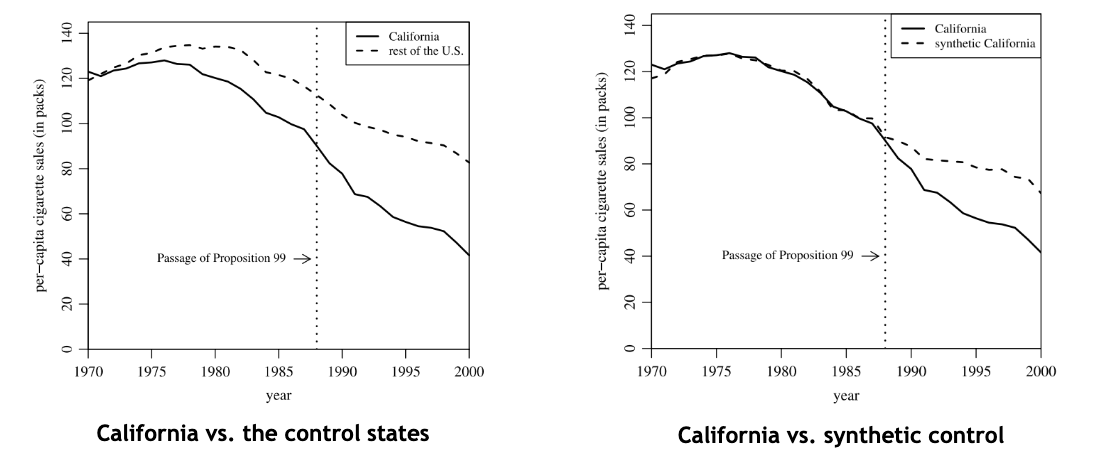
\includegraphics[width=1\textwidth]{2026-04-10-11-20-18.png}
\end{figure}
\newpage 
\subsubsection{Difference (gap) in per-capita cigarette sales}
Only 5 states made up the final synthetic control 
\begin{itemize}
    \item California prior to the treatment is best reproduced by a combination of Colorado, Connecticut, Montana, Nevada and Utah
    \item All other states in the donor pool are assigned zero $W $-weights 
\end{itemize}
\begin{figure}[H]
    \centering
    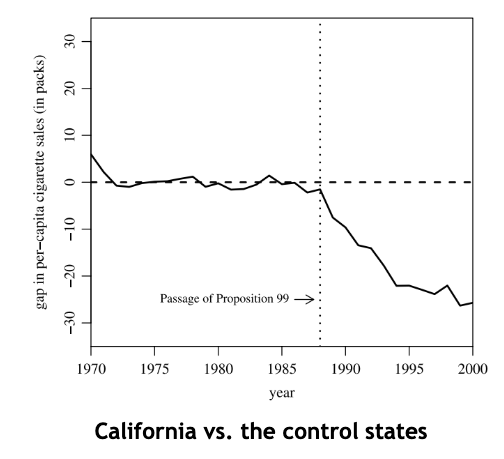
\includegraphics[width=0.5\textwidth]{2026-04-10-11-22-26.png}
\end{figure}
\subsection{Inference}
Traditionally, a form of permutation approach is performed 
\begin{itemize}
    \item Estimte the treatment effect using the same synthetic control procedure using the other control units as treated (i.e., placebo tests)
    \begin{itemize}
        \item If the focal treatment units' effects are unusually large relative to the gaps for the other control units that did not implement treatment, we have confidence in our effect 
        \item However, if other control units can produce similarly large effects, our focal treatment effect might just be caused by random chance 
    \end{itemize}
\end{itemize}
\end{document}